\documentclass[tikz,border=2pt]{standalone}
\usepackage{amsmath,amssymb}
\usepackage{tikz}

\begin{document}
% Dijkstra-Prim: grow the tree from one vertex, each time adding the shortest edge that leaves
% the current tree U; from A the order is A-C, C-B, B-D, D-E, E-F.
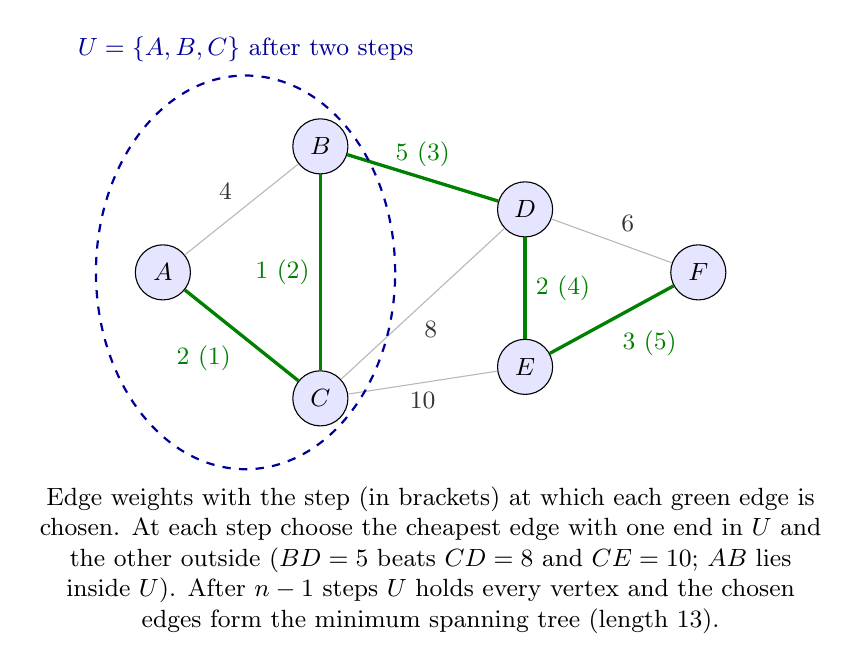
\begin{tikzpicture}[every node/.style={font=\small}, v/.style={draw, circle, fill=blue!10, minimum size=7mm, inner sep=0pt}]
	\node[v] (A) at (0,0) {$A$};
	\node[v] (B) at (2,1.6) {$B$};
	\node[v] (C) at (2,-1.6) {$C$};
	\node[v] (D) at (4.6,0.8) {$D$};
	\node[v] (E) at (4.6,-1.2) {$E$};
	\node[v] (F) at (6.8,0) {$F$};
	\draw[gray!55] (A) -- (B) node[midway, above left, text=gray!40!black] {$4$};
	\draw[gray!55] (C) -- (D) node[pos=0.45, below right, text=gray!40!black] {$8$};
	\draw[gray!55] (C) -- (E) node[midway, below, text=gray!40!black] {$10$};
	\draw[gray!55] (D) -- (F) node[midway, above right, text=gray!40!black] {$6$};
	\draw[green!50!black, very thick] (A) -- (C) node[midway, below left] {$2$ (1)};
	\draw[green!50!black, very thick] (C) -- (B) node[midway, left] {$1$ (2)};
	\draw[green!50!black, very thick] (B) -- (D) node[midway, above] {$5$ (3)};
	\draw[green!50!black, very thick] (D) -- (E) node[midway, right] {$2$ (4)};
	\draw[green!50!black, very thick] (E) -- (F) node[midway, below right] {$3$ (5)};
	\draw[blue!60!black, dashed, thick] (1.05,0.0) ellipse (1.9 and 2.5);
	\node[blue!60!black, anchor=south] at (1.05,2.55) {$U=\{A,B,C\}$ after two steps};
	\node[anchor=north, align=flush center, text width=10cm] at (3.4,-2.6) {Edge weights with the step (in brackets) at which each green edge is chosen. At each step choose the cheapest edge with one end in $U$ and the other outside ($BD=5$ beats $CD=8$ and $CE=10$; $AB$ lies inside $U$). After $n-1$ steps $U$ holds every vertex and the chosen edges form the minimum spanning tree (length $13$).};
\end{tikzpicture}
\end{document}
